 \documentclass{beamer}
\usetheme{Berlin}
\usecolortheme{beaver}
\usepackage[ngerman]{babel}
\usepackage{graphicx}
\usepackage[utf8]{inputenc}
\usepackage{times}
\usepackage[T1]{fontenc}
\usepackage{subfigure}

\title{Imageprocessing - Edge Histograms}
\author{}
\date{}

\begin{document}

\begin{frame}
	\frametitle{Inhalt}
	\begin{enumerate}
		\item Edge Detection
	\end{enumerate}
\end{frame}


\section{Edge Detection}
\begin{frame}
		\begin{block}{Edges:}
			Edges are pixels, in which the image intensity function changes its
			magnitude
		\end{block}
	\begin{figure} 
		\subfigure[Original Image]{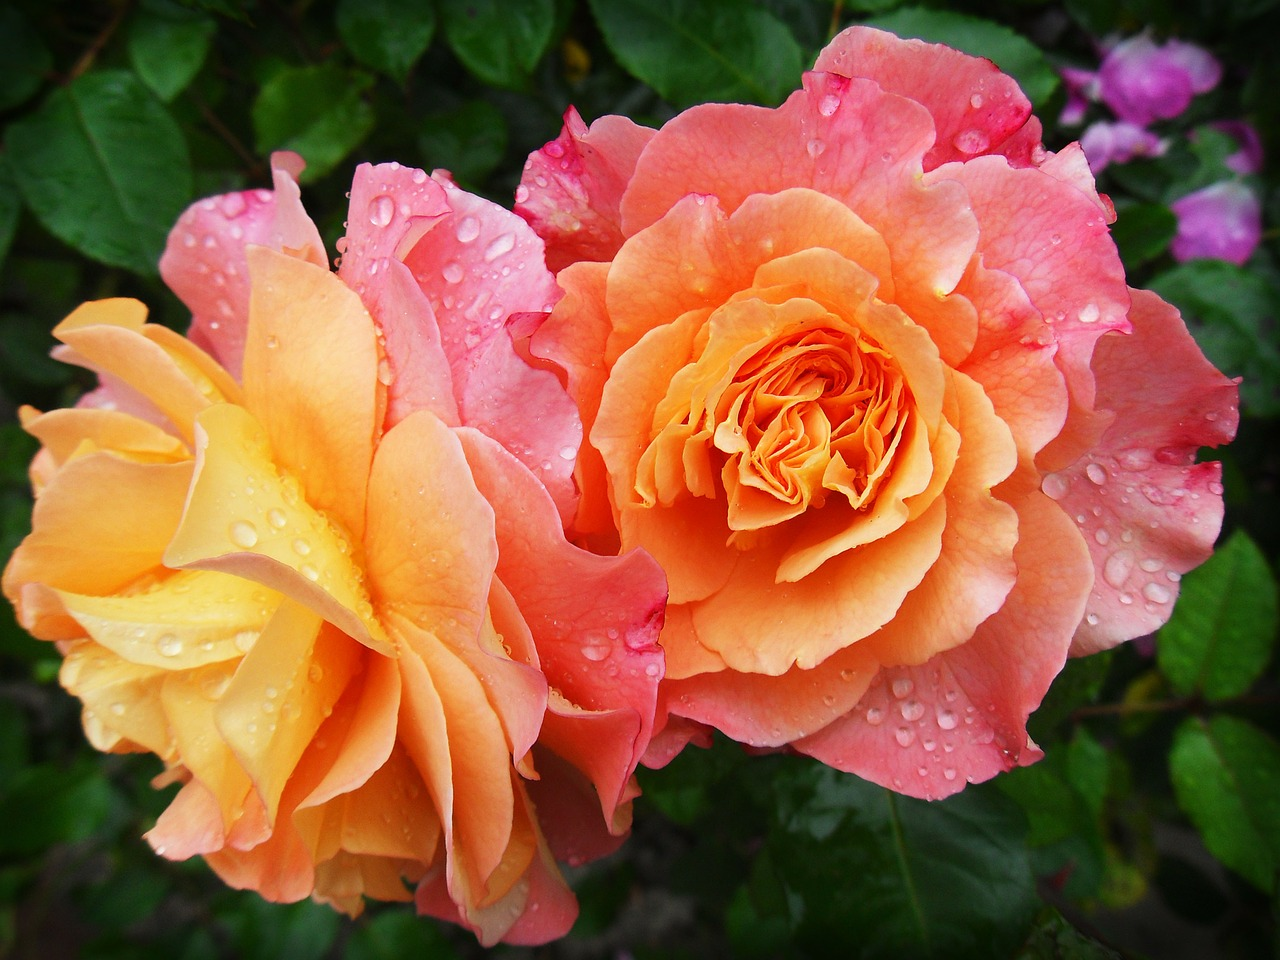
\includegraphics[width=0.49\textwidth]{edge1.jpg}} 
		\subfigure[Image after Edge Detection]{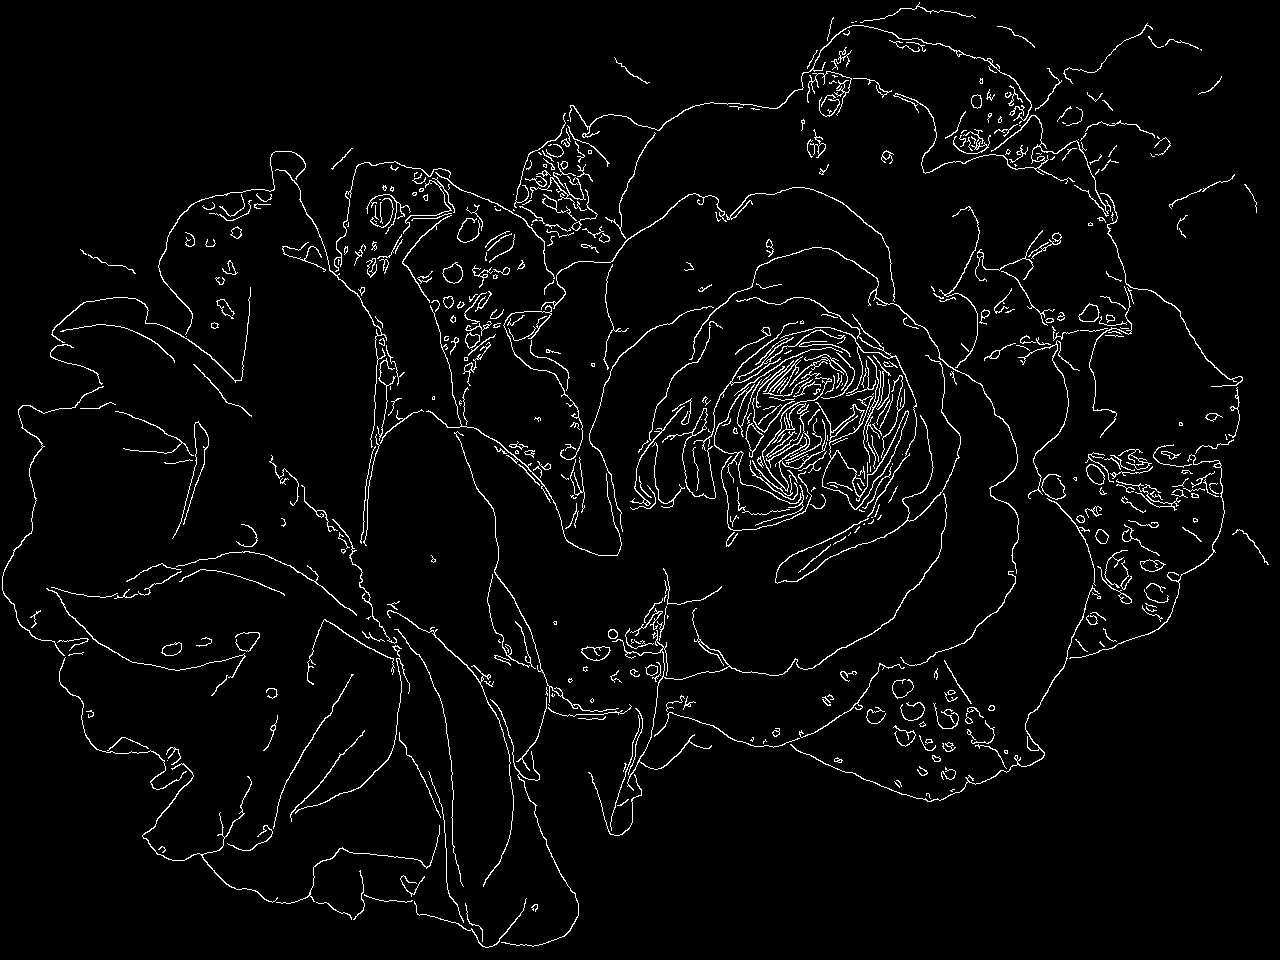
\includegraphics[width=0.49\textwidth]{edge2.jpg}} 
		\caption{Edge Detection using Canny} 
		\end{figure}
\end{frame}

\begin{frame}
	\begin{block}{Edge Detection:}
		Almost every Edge Detector uses either the first derivative or the second derivative of the intensity function. 
	\end{block}
	\begin{figure} 
		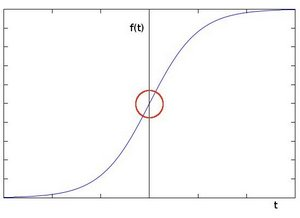
\includegraphics[width=0.49\textwidth]{edge3.jpg}
		\caption{Intensity function} 
	\end{figure}
\end{frame}

\begin{frame}
	\begin{block}{First Derivative:}
		Sobel-, Roberts-, Robinson-, Kirsch-Operator 
	\end{block}
	\begin{figure} 
		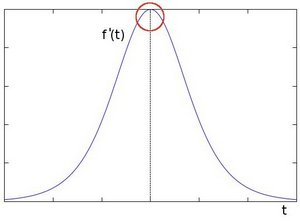
\includegraphics[width=0.49\textwidth]{edge4.jpg}
		\caption{Intensity function - First derivative} 
	\end{figure}
\end{frame}

\begin{frame}
	\begin{block}{Second Derivative:}
	Laplace-, Mexican-Hat-Operator 
	\end{block}
	\begin{figure} 
		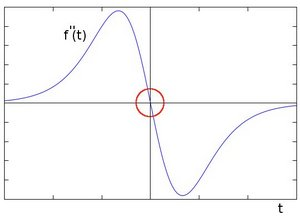
\includegraphics[width=0.49\textwidth]{edge5.jpg}
		\caption{Intensity function - Second derivative} 
	\end{figure}
\end{frame}

\begin{frame}
	\begin{block}{Canny Edge Detection:}
		\begin{itemize}
			\item Low error rate
			\item Good localization
			\item Minimal response
		\end{itemize}
	\end{block}
\end{frame}

\begin{frame}
	\begin{block}{Steps:}
		\begin{enumerate}
			\item Filter out noise using Gaussian filter
			\item Find the intensity gradient using Sobel-Operator\\
			$G = \sqrt{G_x^2 + G_y^2}$ or  $G = |G_x| + |G_y|$
			\item Non-maximum suppression
			\item Hysteresis
		\end{enumerate}
	\end{block}
\end{frame}

\end{document}
